\chapter{Infrared Spectroscopy}\label{ch:g11:infrared}

On a laboratory shelf stands a bottle of colourless liquid whose label
has been torn off. It might be an \omterm{def:g11:functional-groups:alcohol}{alcohol}, a \omterm{def:g11:functional-groups:carbonyl}{ketone} or an acid: three
families that look exactly alike in a bottle. A drop placed on the
crystal of an infrared spectrometer, two minutes of waiting, and a graph
appears on the screen that answers the question. The bonds of a \omterm{def:g7:atoms-and-molecules:molecule}{molecule}
vibrate, and each kind of bond absorbs infrared light of its own
frequencies: an \omterm{def:g11:infrared:spectrum}{infrared spectrum} is a list of the bonds present.

\begin{recall}
\omterm{def:g11:functional-groups:functional-group}{Functional groups} and families (\cref{ch:g11:functional-groups}). An
\omterm{def:g11:absorbance:spectrum}{absorption spectrum} shows how much light a substance absorbs at each
wavelength (\cref{ch:g11:absorbance}). \omterm{def:g11:polarity-and-cohesion:hydrogen-bond}{Hydrogen bonds} link \ce{O-H}
groups to neighbouring \omterm{def:g7:atoms-and-molecules:molecule}{molecules} (\cref{ch:g11:polarity-and-cohesion}).
\end{recall}

\section{Bonds vibrate}

A \omterm{def:g10:lewis-and-shape:covalent-bond}{covalent bond} is not rigid: the two \omterm{def:g7:atoms-and-molecules:atom}{atoms} vibrate, moving closer and
apart many millions of millions of times per second, like two balls
joined by a spring. A stiffer spring (a \omterm{def:g10:lewis-and-shape:multiple-bond}{double bond} rather than a single
one) or lighter balls (a hydrogen \omterm{def:g7:atoms-and-molecules:atom}{atom} rather than a carbon \omterm{def:g7:atoms-and-molecules:atom}{atom}) vibrate
faster. A bond can absorb infrared light whose frequency matches its own
vibration: infrared light, invisible to the eye, has wavelengths of a few
micrometres to a few tens of micrometres.

\begin{omfigure}
\begin{tikzpicture}[font=\small]
  \node[aC] (c) at (0,0) {};
  \node[aO] (o) at (2.2,0) {};
  \draw[decorate, decoration={coil, aspect=0.4, segment length=4pt,
    amplitude=4pt}, thick, black!60] (c.east) -- (o.west);
  \draw[<->, omProp, thick] (-0.9,0) -- (-0.45,0);
  \draw[<->, omProp, thick] (2.65,0) -- (3.1,0);
  \node[anchor=north] at (1.1,-0.5) {a bond stretching and shrinking};
  \node[aO] (o1) at (5.3,0) {};
  \node[aH] (h1) at (6.7,0) {};
  \draw[decorate, decoration={coil, aspect=0.4, segment length=3pt,
    amplitude=3pt}, thick, black!60] (o1.east) -- (h1.west);
  \draw[<->, omProp, thick] (7.0,0) -- (7.7,0);
  \node[anchor=north, align=center] at (6.2,-0.5) {a light hydrogen atom:\\ faster vibration};
\end{tikzpicture}

{\small A bond pictured as a spring between two balls. Its vibration has
a frequency set by the stiffness of the bond and the masses of the \omterm{def:g7:atoms-and-molecules:atom}{atoms};
infrared light of that frequency is absorbed.}
\end{omfigure}

\begin{definition}[Wavenumber]\label{def:g11:infrared:wavenumber}
The \emph{wavenumber}\index{wavenumber} $\sigma$ of a light is the
inverse of its wavelength, $\sigma = 1/\lambda$. In infrared
spectroscopy it is expressed in \si{cm^{-1}}: the number of wavelengths
in one centimetre. A larger wavenumber means a shorter wavelength and a
faster vibration.
\end{definition}

\begin{example}[From a wavenumber to a wavelength]\label{ex:g11:infrared:convert}
A band at $\sigma = \qty{2000}{cm^{-1}}$ corresponds to
$\lambda = 1/2000 = \qty{5.0e-4}{cm} = \qty{5.0}{\micro m}$. Infrared
spectra usually run from \qty{4000}{cm^{-1}} (\qty{2.5}{\micro m}) to
\qty{500}{cm^{-1}} (\qty{20}{\micro m}).
\end{example}

\section{Reading an infrared spectrum}

\begin{definition}[Infrared spectrum, transmittance]\label{def:g11:infrared:spectrum}
The \emph{transmittance}\index{transmittance} $T$ of a sample at a given
\omterm{def:g11:infrared:wavenumber}{wavenumber} is the percentage of the infrared light that passes through
it: \qty{100}{\percent} if nothing is absorbed. The \emph{infrared
spectrum}\index{infrared spectrum} of a compound is the graph of $T$
against the \omterm{def:g11:infrared:wavenumber}{wavenumber}, drawn by convention with the \omterm{def:g11:infrared:wavenumber}{wavenumbers}
decreasing from left to right.
\end{definition}

\begin{definition}[Absorption band, fingerprint region]\label{def:g11:infrared:band}
An \emph{absorption band}\index{absorption band} is a dip of the
\omterm{def:g11:infrared:spectrum}{transmittance}: the light of those \omterm{def:g11:infrared:wavenumber}{wavenumbers} is absorbed by a bond. Its
position tells which bond, its width and its depth complete the
picture. Below about \qty{1500}{cm^{-1}}, the spectrum is crowded with
bands that depend on the whole \omterm{def:g7:atoms-and-molecules:molecule}{molecule}: this \emph{fingerprint
region}\index{fingerprint region} identifies a compound by comparison
with a known spectrum, but is hard to read bond by bond.
\end{definition}

\begin{inthelab}[Recording a spectrum]
Most school and university spectrometers now use a small diamond crystal:
a drop of liquid, or a few grains of solid pressed by a clamp, is placed
on the crystal, and the infrared beam that grazes its surface probes the
sample. The crystal is first recorded clean (the ``background''), which
plays the part of the blank. The crystal is cleaned with a tissue and a
little \omterm{def:g6:solutions-and-solubility:solute}{solvent} between two samples.
\end{inthelab}

\section{Characteristic bands}

\begin{proposition}[Each bond type has its band]\label{prop:g11:infrared:bands}
% ledger: ir:OH-free, ir:OH-bonded, ir:OH-acid, ir:NH, ir:CH, ir:CO-aldehyde, ir:CO-ketone, ir:CO-ester, ir:CO-acid, ir:CC-double, ir:CO-single
Each type of bond absorbs in a characteristic range of \omterm{def:g11:infrared:wavenumber}{wavenumbers},
nearly the same from one \omterm{def:g7:atoms-and-molecules:molecule}{molecule} to the next:
\begin{center}
\small
\begin{tabular}{lll}
\hline
bond & \omterm{def:g11:infrared:wavenumber}{wavenumber} (\si{cm^{-1}}) & appearance \\
\hline
\ce{O-H}, not hydrogen-bonded (gas, dilute) & near 3600 & sharp \\
\ce{O-H}, hydrogen-bonded (liquid \omterm{def:g11:functional-groups:alcohol}{alcohol}) & 3300--3400 & broad, strong \\
\ce{O-H} of a \omterm{def:g11:functional-groups:carboxylic-acid}{carboxylic acid} & 2500--3300 & very broad \\
\ce{N-H} of an \omterm{def:g11:functional-groups:amine}{amine} & 3300--3500 & medium (two bands for \ce{-NH2}) \\
\ce{C-H} of a chain & 2850--2960 & strong \\
\ce{C=O} of an \omterm{def:g11:functional-groups:carboxylic-acid}{ester} & near 1735 & very strong, sharp \\
\ce{C=O} of an \omterm{def:g11:functional-groups:carbonyl}{aldehyde} & near 1730 & very strong, sharp \\
\ce{C=O} of a \omterm{def:g11:functional-groups:carbonyl}{ketone} & near 1715 & very strong, sharp \\
\ce{C=O} of a \omterm{def:g11:functional-groups:carboxylic-acid}{carboxylic acid} & near 1710 & very strong, broader \\
\ce{C=C} & near 1650 & medium \\
\ce{C-O} of an \omterm{def:g11:functional-groups:alcohol}{alcohol} & near 1050 & strong \\
\hline
\end{tabular}
\end{center}
\end{proposition}

\begin{proof}
These ranges are measured on many compounds (ledger). They group by
bond because the vibration of a bond depends mostly on the bond itself
and its two \omterm{def:g7:atoms-and-molecules:atom}{atoms}, little on the rest of the \omterm{def:g7:atoms-and-molecules:molecule}{molecule}.
\end{proof}

\begin{omfigure}
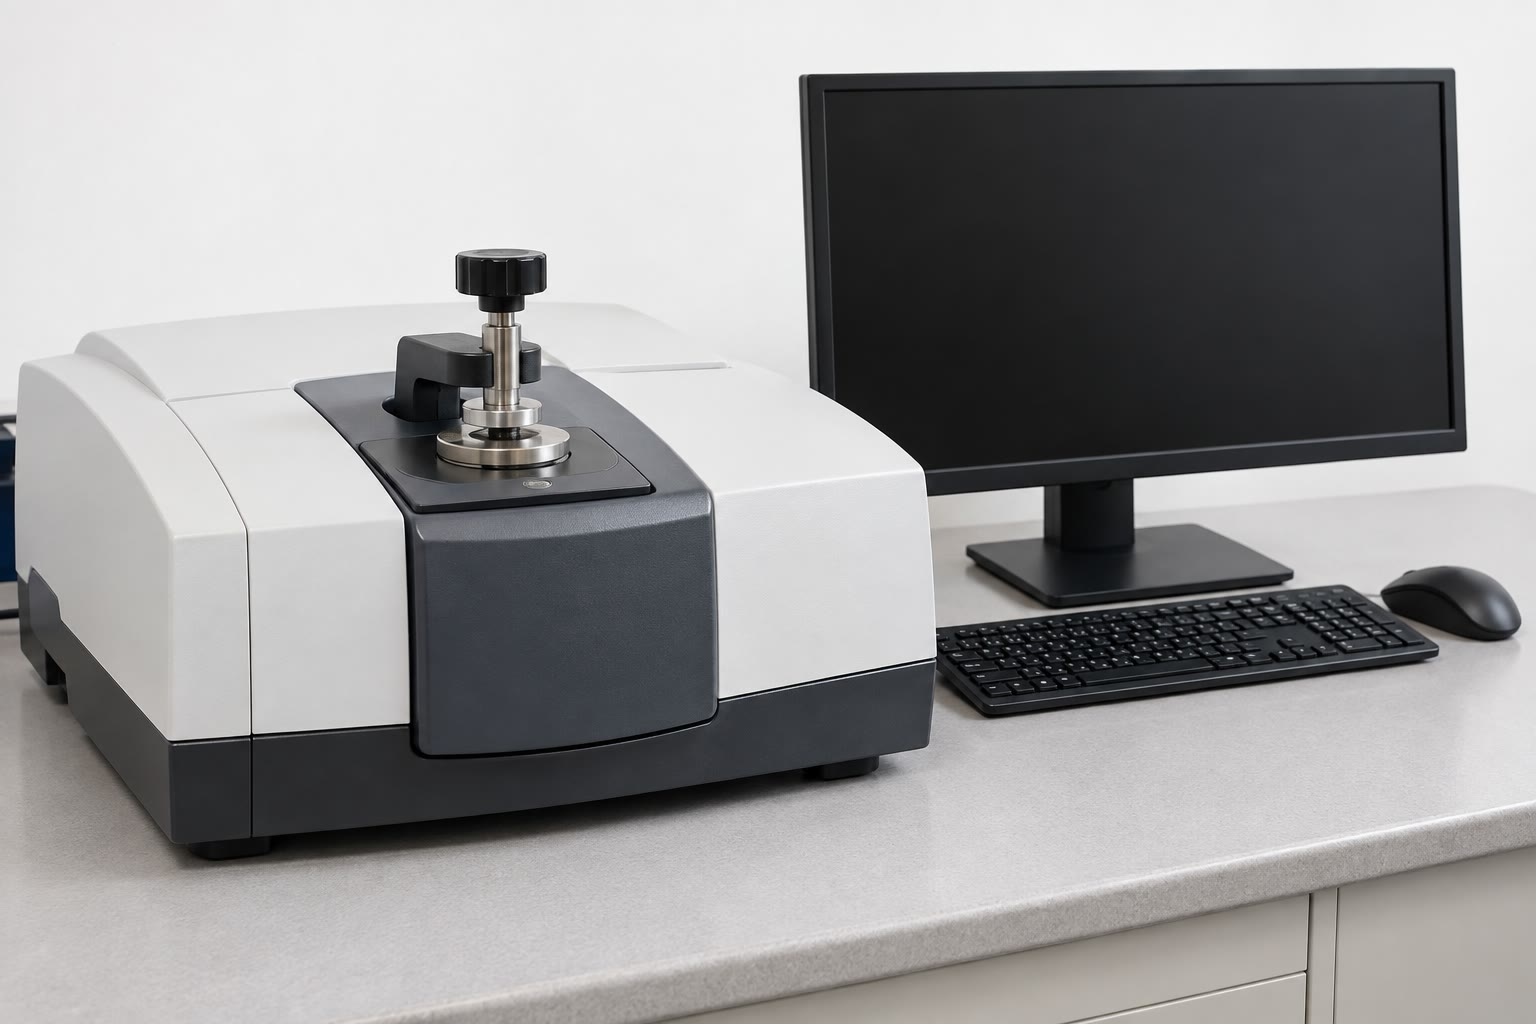
\includegraphics[width=0.48\linewidth]{images/book1/ai/g11-ftir.jpg}

{\small A benchtop infrared spectrometer with its crystal and clamp.}
\end{omfigure}

\begin{omfigure}
\begin{tikzpicture}[font=\small, x=0.0036cm, y=0.5cm]
  % wavenumber axis reversed: x = 4000 - sigma
  \fill[black!8] (2500,0.2) rectangle (3500,7.6);
  \node[font=\footnotesize, align=center, black!60] at (3000,6.8) {fingerprint\\ region};
  \draw[->] (0,0) -- (3600,0) node[right] {$\sigma$};
  \foreach \s in {4000,3500,3000,2500,2000,1500,1000,500}
    \draw ({4000-\s},0) -- ({4000-\s},-0.15) node[below, font=\footnotesize] {\s};
  \node[below=12pt] at (1800,-0.3) {wavenumber (\si{cm^{-1}})};
  \foreach \a/\b/\y/\c/\l in {
      3600/3600/7/omDef/{\ce{O-H} free},
      3300/3400/6/omDef/{\ce{O-H} bonded},
      2500/3300/5/omThm/{\ce{O-H} acid},
      3300/3500/4/omMeth/{\ce{N-H}},
      2850/2960/3/black!60/{\ce{C-H}},
      1700/1740/2/omProp/{\ce{C=O}},
      1050/1050/1/black!45/{\ce{C-O}}} {
    \fill[\c, rounded corners=1pt] ({4000-\b-12},{\y-0.25}) rectangle ({4000-\a+12},{\y+0.25});
    \node[anchor=west, font=\footnotesize] at ({4000-\a+40},\y) {\l};
  }
\end{tikzpicture}

{\small Where the main bonds absorb. The \ce{O-H} and \ce{N-H} bands sit
at the left, the \ce{C=O} band, usually the strongest, near
\qty{1700}{cm^{-1}}; below \qty{1500}{cm^{-1}} lies the \omterm{def:g11:infrared:band}{fingerprint
region}.}
\end{omfigure}

\begin{proposition}[Hydrogen bonds broaden the O--H band]\label{prop:g11:infrared:hbond}
% ledger: ir:OH-free, ir:OH-bonded, ir:ethanol-OH
When \ce{O-H} groups are linked by \omterm{def:g11:polarity-and-cohesion:hydrogen-bond}{hydrogen bonds}, as in a liquid
\omterm{def:g11:functional-groups:alcohol}{alcohol}, their band is broad and lies at lower \omterm{def:g11:infrared:wavenumber}{wavenumbers} (about
3300--\qty{3400}{cm^{-1}}); without \omterm{def:g11:polarity-and-cohesion:hydrogen-bond}{hydrogen bonds}, as in the gas, it is
sharp and near \qty{3600}{cm^{-1}}.
\end{proposition}

\begin{proof}
Admitted: a \omterm{def:g11:polarity-and-cohesion:hydrogen-bond}{hydrogen bond} pulls on the hydrogen \omterm{def:g7:atoms-and-molecules:atom}{atom} and loosens the
\ce{O-H} bond, which vibrates more slowly; and since every \omterm{def:g7:atoms-and-molecules:molecule}{molecule} is
bonded a little differently, the band spreads over a range.
\end{proof}

\section{Identifying functional groups}


\begin{method}[Reading an infrared spectrum]\label{met:g11:infrared:reading}
\begin{enumerate}
  \item Look above \qty{1500}{cm^{-1}} first; leave the \omterm{def:g11:infrared:band}{fingerprint
        region} for a comparison with known spectra.
  \item Near \qty{1700}{cm^{-1}}: a very strong band means a \ce{C=O}
        group (\omterm{def:g11:functional-groups:carbonyl}{aldehyde}, \omterm{def:g11:functional-groups:carbonyl}{ketone}, acid, \omterm{def:g11:functional-groups:carboxylic-acid}{ester}, \omterm{def:g11:functional-groups:amine}{amide}).
  \item Between 2500 and \qty{3700}{cm^{-1}}: a broad band near
        \qty{3350}{cm^{-1}} means an \omterm{def:g11:functional-groups:alcohol}{alcohol} \ce{O-H}; a very broad band
        from 2500 to \qty{3300}{cm^{-1}} with a \ce{C=O} means a
        \omterm{def:g11:functional-groups:carboxylic-acid}{carboxylic acid}; medium bands at 3300--\qty{3500}{cm^{-1}} mean
        \ce{N-H}.
  \item Combine with the \omterm{def:g11:organic-skeletons:formulas}{molecular formula} to choose the family, then
        check with the position of the \ce{C=O} band if there is one.
\end{enumerate}
\end{method}

\begin{omfigure}
\newcommand{\irpanel}[2]{%
\begin{tikzpicture}
\begin{axis}[width=0.96\linewidth, height=3.9cm, x dir=reverse, xmin=500,
    xmax=4000, ymin=0, ymax=105, xtick={4000,3000,2000,1000},
    /pgf/number format/1000 sep={},
    ytick={0,50,100}, tick label style={font=\scriptsize},
    label style={font=\scriptsize}, ylabel={$T$ (\%)}, axis lines*=left,
    title={\small #2}, title style={yshift=-4pt}]
  \addplot[thick, omDef] table[x=sigma, y=#1] {figdata/out/grade-11-infrared.dat};
\end{axis}
\end{tikzpicture}}
\begin{minipage}{0.49\linewidth}\irpanel{ethanolL}{A: ethanol (liquid)}\end{minipage}\hfill
\begin{minipage}{0.49\linewidth}\irpanel{ethanolG}{B: ethanol (gas)}\end{minipage}

\begin{minipage}{0.49\linewidth}\irpanel{propanone}{C: propanone}\end{minipage}\hfill
\begin{minipage}{0.49\linewidth}\irpanel{acid}{D: ethanoic acid}\end{minipage}

\begin{minipage}{0.49\linewidth}\irpanel{ester}{E: ethyl ethanoate}\end{minipage}\hfill
\begin{minipage}{0.49\linewidth}\irpanel{amine}{F: ethanamine}\end{minipage}

{\small Infrared spectra of six compounds, \omterm{def:g11:infrared:wavenumber}{wavenumber} in \si{cm^{-1}}
(decreasing to the right). Only the bands discussed in the chapter are
drawn; their positions come from measured spectra and tables, their
shapes from a simple model.}
\end{omfigure}

\begin{example}[Reading the six spectra]\label{ex:g11:infrared:six}
% ledger: ir:OH-bonded, ir:ethanol-OH, ir:CO-ketone, ir:OH-acid, ir:CO-acid, ir:CO-ester, ir:ethylethanoate-COC, ir:NH
Ethanol (A) shows a broad \ce{O-H} band near \qty{3350}{cm^{-1}}, the
\ce{C-H} bands just below \qty{3000}{cm^{-1}} and a strong \ce{C-O} band
near \qty{1050}{cm^{-1}}, but nothing near \qty{1700}{cm^{-1}}. In the
gas (B), its \ce{O-H} band becomes a sharp line at
\qty{3666}{cm^{-1}}. Propanone (C) has no \ce{O-H} band but a very strong
\ce{C=O} at \qty{1715}{cm^{-1}}. Ethanoic acid (D) shows both: an
enormous \ce{O-H} band from 2500 to \qty{3300}{cm^{-1}} and a \ce{C=O}
at \qty{1710}{cm^{-1}}. Ethyl ethanoate (E) has its \ce{C=O} at
\qty{1735}{cm^{-1}} and a strong \ce{C-O} near \qty{1240}{cm^{-1}}, and
no \ce{O-H}. Ethanamine (F) shows two medium \ce{N-H} bands above
\qty{3300}{cm^{-1}}.
\end{example}

\section{Exercises}

\begin{exercise}[$\star$]\label{exo:g11:infrared:1}
Convert into a wavelength in micrometres: $\sigma = \qty{3300}{cm^{-1}}$
and $\sigma = \qty{1050}{cm^{-1}}$. Which corresponds to the faster
vibration?
\end{exercise}

\begin{exercise}[$\star$]\label{exo:g11:infrared:2}
A wavelength of \qty{10}{\micro m} is absorbed. Give the \omterm{def:g11:infrared:wavenumber}{wavenumber} in
\si{cm^{-1}}.
\end{exercise}

\begin{exercise}[$\star$]\label{exo:g11:infrared:3}
Which bond absorbs: near \qty{1715}{cm^{-1}}; near \qty{3350}{cm^{-1}}
(broad); between 2850 and \qty{2960}{cm^{-1}}?
\end{exercise}

\begin{exercise}[$\star$]\label{exo:g11:infrared:4}
On spectrum C (propanone), find the strongest band. Which bond does it
belong to?
\end{exercise}

\begin{exercise}[$\star$]\label{exo:g11:infrared:5}
Why is an \omterm{def:g11:infrared:spectrum}{infrared spectrum} drawn with a \omterm{def:g11:infrared:spectrum}{transmittance} axis, the bands
pointing down? What does $T = \qty{100}{\percent}$ mean?
\end{exercise}

\begin{exercise}[$\star\star$]\label{exo:g11:infrared:6}
A compound \ce{C4H8O} shows a very strong band at
\qty{1715}{cm^{-1}} and no band above \qty{3000}{cm^{-1}}. Another,
\ce{C4H10O}, shows a broad band near \qty{3350}{cm^{-1}} and none near
\qty{1700}{cm^{-1}}. To which families do they belong? Propose a name
for each.
\end{exercise}

\begin{exercise}[$\star\star$]\label{exo:g11:infrared:7}
Explain why the \ce{O-H} band of ethanoic acid is so broad, broader even
than that of liquid ethanol.
\end{exercise}

\begin{exercise}[$\star\star$]\label{exo:g11:infrared:8}
Compare spectra A and B of ethanol. What changes, and why?
\end{exercise}

\begin{exercise}[$\star\star$]\label{exo:g11:infrared:9}
Propanal and propanone are both \ce{C3H6O}. Both show a strong \ce{C=O}
band. Can infrared tell them apart from that band alone? What else could
help?
\end{exercise}

\begin{exercise}[$\star\star$]\label{exo:g11:infrared:10}
A compound shows a strong band at \qty{1735}{cm^{-1}}, a strong band near
\qty{1240}{cm^{-1}} and nothing above \qty{3000}{cm^{-1}}. Its formula is
\ce{C4H8O2}. Which family? Is ethanoic acid a possibility? Butanoic
acid?
\end{exercise}

\begin{exercise}[$\star\star$]\label{exo:g11:infrared:11}
Which of the six spectra would a \omterm{def:g7:atoms-and-molecules:molecule}{molecule} of propan-1-ol most resemble?
Of propanoic acid? Explain.
\end{exercise}

\begin{exercise}[$\star\star\star$]\label{exo:g11:infrared:12}
Propan-2-ol can be oxidised into propanone. A student follows the
reaction by recording spectra of samples taken every ten minutes.
Describe how the spectra change. How does she know the reaction is
complete?
\end{exercise}

\begin{exercise}[$\star\star\star$]\label{exo:g11:infrared:13}
Butanoic acid and ethyl ethanoate are \omterm{def:g11:organic-skeletons:isomer}{isomers}, \ce{C4H8O2}. Describe two
differences between their infrared spectra, and explain them.
\end{exercise}

\begin{exercise}[$\star\star\star$]\label{exo:g11:infrared:14}
A sample of ethyl ethanoate shows, besides the expected bands, a weak
broad band near \qty{3350}{cm^{-1}}. Suggest two impurities that could
cause it (think of how \omterm{def:g11:functional-groups:carboxylic-acid}{esters} are made, and of the \omterm{def:g4:air-a-mixture-of-gases:air}{air}). How could the
sample be checked?
\end{exercise}

\begin{exercise}[$\star\star\star$]\label{exo:g11:infrared:15}
The \ce{C=O} band of \omterm{def:g11:functional-groups:carbonyl}{ketones} lies near \qty{1715}{cm^{-1}}, that of a
\ce{C=C} near \qty{1650}{cm^{-1}}, and the \ce{C-O} band near
\qty{1050}{cm^{-1}}. Using the picture of two balls on a spring, explain
why a \omterm{def:g10:lewis-and-shape:multiple-bond}{double bond} \ce{C=O} vibrates faster than a single bond \ce{C-O}.
Why are \ce{O-H}, \ce{N-H} and \ce{C-H} bands all at high \omterm{def:g11:infrared:wavenumber}{wavenumbers}?
\end{exercise}

\section{Problem: Three Unlabelled Bottles}

\begin{problem}[{Weekend problem --- three bottles have lost their labels:
which is which, and what wavelength does the ketone absorb most?}]
\label{pb:g11:infrared:1}
% ledger: ir:OH-bonded, ir:OH-acid, ir:CO-ketone, ir:CO-acid, ir:CO-single
Three bottles of colourless liquid have lost their labels. The stock list
says they contain ethanol, propanone and ethanoic acid. Their spectra are
recorded: bottle 1 gives a spectrum like A, bottle 2 like D, bottle 3
like C.

\medskip
\noindent\textbf{Part I --- The candidates.}
\begin{enumerate}
  \item Write the \omterm{def:g11:organic-skeletons:formulas}{semi-structural formulas} of ethanol, propanone and
        ethanoic acid.
  \item Give their \omterm{def:g11:organic-skeletons:formulas}{molecular formulas}.
  \item Name the \omterm{def:g11:functional-groups:functional-group}{functional group} of each.
  \item Which bonds of each should give a band above
        \qty{1500}{cm^{-1}}?
\end{enumerate}

\medskip
\noindent\textbf{Part II --- The spectra.}
\begin{enumerate}[resume]
  \item Bottle 1: is there a \ce{C=O} band? An \ce{O-H} band? Which
        compound is it?
  \item Bottle 2: describe its two strongest features. Which compound?
  \item Bottle 3: which compound? Which band decides?
  \item Could the smell have told them apart? Why is it better not to
        try?
  \item Why is the \ce{O-H} band of bottle 2 wider than that of bottle 1?
\end{enumerate}

\medskip
\noindent\textbf{Part III --- \omterm{def:g11:organic-skeletons:isomer}{Isomers}.}
\begin{enumerate}[resume]
  \item Methoxymethane is an isomer of ethanol. Write its formula. Which
        band of ethanol would its spectrum lack?
  \item Propanal is an isomer of propanone. Which band do they share?
        Where does it lie for each?
  \item Methyl methanoate, \ce{HCOO-CH3}, is an isomer of ethanoic acid.
        Which band of the acid would be missing? Where would its
        \ce{C=O} band lie?
  \item Why can a \omterm{def:g11:organic-skeletons:formulas}{molecular formula} alone not identify a compound, while
        formula and spectrum together usually can?
\end{enumerate}

\medskip
\noindent\textbf{Part IV --- The wavelength.}
\begin{enumerate}[resume]
  \item What is the \omterm{def:g11:infrared:wavenumber}{wavenumber} of the strongest band of propanone?
  \item Express it in \si{m^{-1}}.
  \item Compute the wavelength absorbed, in metres, then in
        micrometres.
  \item Is that light visible? To which kind of radiation does it
        belong?
  \item Do the same for the \ce{C-O} band of ethanol near
        \qty{1050}{cm^{-1}}.
  \item Which of the two bonds vibrates faster?
  \item State the final answer: what wavelength does the \ce{C=O} bond of
        propanone absorb most strongly?
\end{enumerate}
\end{problem}
